\documentclass[11pt]{article}

% ======================================================================
% Comprehensive technical report for the FINAL bruise-segmentation run
% (bruise_colab_final.ipynb) and its analysis (bruise_colab_final_analysis.ipynb).
% Self-contained: standard article class, no external .sty beyond CTAN packages,
% so it compiles with a portable Tectonic:
%     tools/tectonic/tectonic.exe docs/final_run_report.tex
% Baseline architectures (U-Net / DeepLabV3+ / nnU-Net) will be added later;
% Section 9 is a stub reserved for them.
% ======================================================================

\usepackage[margin=1in]{geometry}
\usepackage{booktabs}
\usepackage{amsmath,amssymb}
\usepackage{graphicx}
\usepackage{xcolor}
\usepackage{siunitx}
\usepackage{caption}
\usepackage{enumitem}
\usepackage[hidelinks]{hyperref}
\usepackage{titlesec}

\sisetup{detect-weight=true, round-mode=places, round-precision=3}
\newcommand{\best}[1]{\textbf{#1}}
\newcommand{\sig}{\textcolor{red!70!black}{\textbf{significant}}}
\newcommand{\ns}{n.s.}

\titleformat{\section}{\normalfont\Large\bfseries}{\thesection}{0.6em}{}
\setlength{\parskip}{0.4em}
\setlength{\parindent}{0pt}

\title{\bfseries Distillation, Failure Modes, and Benchmark Fragility in\\
Forensic White-Light Bruise Segmentation:\\
\large A Comprehensive Report on the Final Five-Model Run}
\author{Injury Analytics Lab --- Bruise Segmentation Project}
\date{Generated from \texttt{results\_final/} and the val-selected best-seed re-inference\\
(final run: \texttt{bruise\_colab\_final.ipynb}; analysis: \texttt{bruise\_colab\_final\_analysis.ipynb})}

\begin{document}
\maketitle

\begin{abstract}
\noindent
We report a controlled comparison of five semantic-segmentation models for
white-light (WL) bruise segmentation on a multi-annotator forensic dataset: a
SegFormer-B2 teacher, a SegFormer-B0 student trained directly, a SegFormer-B0
student trained with calibrated soft-target distillation, and two YOLO26n-sem
models (direct and distilled) trained with their native Ultralytics recipe. All
models are trained only on one annotator's masks and evaluated against a
three-annotator \emph{majority-vote} target on a fixed test set of
\textbf{185 images from 28 subjects}. The central quantitative facts are: (i) at
28 subjects the minimum resolvable difference in mean Dice is $\approx 0.04$,
which is \emph{larger} than the distillation effect ($+0.002$, \ns) and the
student--teacher gap ($-0.001$, \ns); (ii) the one axis that separates the
architectures by more than label noise is the \emph{complete-miss rate}
(SegFormer $0$--$0.5\%$ vs.\ YOLO $2$--$8\%$); (iii) the three human experts agree
with one another at only \textbf{0.639} mean Dice, and every model beats that
ceiling---indeed a model trained on a single annotator (Paul) agrees with the
three-expert consensus \emph{significantly better than Paul himself does}
($+0.07$ Dice, $P(\Delta{>}0)\approx0.98$); and (iv) an apparent skin-tone
performance gap is confounded with lesion size, though a residual light-skin
recall deficit for YOLO survives adjustment for size and subject clustering at
the boundary of significance ($p\approx0.05$). We frame the study as a case
study in benchmark fragility: the conclusions turn far more on annotation noise,
sample size, and evaluation-harness choices than on architecture. Two external
baselines (U-Net and DeepLabV3+, ResNet50) trained through the identical recipe land at
$0.753\pm0.015$ and $0.745\pm0.018$ mean Dice---within $\approx$0.02 of the SegFormer
models and well inside the annotation-noise band---so with seven architectures now
clustering at 0.745--0.765, the label-limited reading only strengthens
(Section~\ref{sec:baselines}; nnU-Net still pending).
\end{abstract}

\tableofcontents
\bigskip

% ======================================================================
\section{Introduction}
% ======================================================================
Bruises are central evidence in forensic assessment of physical abuse, yet their
boundaries are diffuse and their appearance varies with skin tone, lighting, age
of injury, and body site. Automated segmentation could standardise documentation,
but it inherits two hard problems: (1) the ``ground truth'' is itself a matter of
expert opinion, and expert opinions disagree; and (2) the population for which
three-expert consensus labels exist is small. This report documents a five-model
run built specifically to be \emph{honest} about both problems---to measure them
rather than to hide them behind a single accuracy number.

We compare a transformer family (SegFormer) against a modern one-stage detector
family (YOLO26n-sem), including knowledge distillation from a large teacher to a
small student in each family. The comparison is deliberately conservative: every
difference is quantified with a \emph{subject-level cluster bootstrap}, and the
headline results are the ones that survive it.

% ======================================================================
\section{Dataset and Experimental Design}
% ======================================================================
\subsection{A multi-annotator intersection study}
The data are white-light photographs from the NIJ bruise dataset, labelled by
multiple annotators. The three highest-volume annotators---\textbf{Paul},
\textbf{Gbarimah}, and \textbf{Erik}---were identified. The \emph{strict
intersection} of all three (every image labelled by all three annotators) is
\textbf{185 white-light images from 28 subjects}, and this intersection
\emph{is} the fixed test set. The prediction target is the per-pixel
\textbf{2-of-3 majority vote} (a pixel is bruise if at least two of the three
annotators marked it), \emph{not} any single annotator's mask.

\subsection{Train/test discipline}
A prior five-fold cross-annotator study selected Paul as the most stable
annotator, so all five models are \textbf{trained only on Paul's masks} and
\textbf{evaluated against the three-annotator majority}. Training data are Paul's
\emph{non-intersection} subjects (831 images / 115 subjects), split
\textbf{697 train / 134 validation} at the subject level. Because the 28 test
subjects are structurally removed from the training pool, subject disjointness is
guaranteed by construction (verified: 0 overlapping subjects). This is a
\emph{cross-annotator generalisation} test, not an ordinary split.

\subsection{$n=28$ is a ceiling, not a choice}
There are 28 test subjects because that is how many subjects \emph{all three}
annotators labelled; a 29th cannot be obtained without new annotation. Every
``underpowered'' statement below should therefore be read as a fact about the
field---\emph{at the maximum sample size for which three-annotator consensus
labels exist, model-level differences are largely unresolvable}---not as a
limitation that more effort could remove.

\subsection{Skin-tone grouping}
For subgroup analysis we use the Individual Typology Angle (ITA), an objective
skin-tone measure computed from image pixels, binned into five Fitzpatrick-like
groups (Light II--III, Intermediate III--IV, Tan IV, Brown V, Dark VI). Group
sizes range from 24 to 55 images but only $\approx$9--17 \emph{subjects}, which
governs the (weak) statistical power of every fairness statement in
Section~\ref{sec:fairness}.

% ======================================================================
\section{Architectures}
% ======================================================================
All five models emit a \emph{single} bruise logit at full input resolution, so
every downstream component (loss, threshold sweep, metric, benchmark) is
architecture-blind.

\subsection{SegFormer (B2 teacher, B0 students)}
HuggingFace SegFormer with a MiT (Mix-Transformer) hierarchical encoder and a
lightweight all-MLP decode head, rebuilt with a 1-class head. Input is
ImageNet-normalised inside the model wrapper. The teacher is \textbf{MiT-B2}
(\num{27347393} parameters, i.e.\ 27.35\,M); both students are \textbf{MiT-B0}
(3.71\,M). The B0 decode head is randomly initialised on a pretrained backbone.

\subsection{YOLO26n-sem}
Ultralytics YOLO26n semantic-segmentation model, rebuilt with an $nc{=}1$ head so
it emits one bruise logit directly (structurally mirroring SegFormer's 1-channel
head). \texttt{.load()} transfers 360/364 backbone tensors; only the head is new.
Input scale is $/255$ (no ImageNet normalisation), because Ultralytics'
BatchNorms carry running statistics for that distribution---feeding it
ImageNet-normalised pixels caps it at Dice 0.479. Parameter count 1.63\,M. A
structural note relevant to the results: YOLO's main head operates at stride 8
($80\times80$ for a $640$ input) against SegFormer's stride 4 ($160\times160$), a
$4\times$ coarser spatial grid that is an architectural ceiling on boundary
precision, not a training artefact.

% ======================================================================
\section{Training and Evaluation Protocol}
% ======================================================================
\subsection{Shared recipe (SegFormer)}
Loss is per-image Dice$+$BCE (Dice computed per image then averaged, to match the
reported metric and to keep gradient on the $\approx$4.7\% of pixels that are
bruise). Optimiser is AdamW with an encoder/head learning-rate split
($6\times10^{-5}$ / $6\times10^{-4}$), no weight decay on norms and biases,
linear warmup then polynomial decay, AMP, and gradient clipping. \textbf{Model
selection is on a threshold-free binned average precision (AP)} over validation
pixels, not on Dice at a fixed 0.5 threshold (the operating threshold is fitted
afterwards and is nowhere near 0.5). After training, the decision threshold is
\textbf{swept on validation and applied once to test}.

\subsection{Distillation (what it is, and is not)}
The distilled models use \emph{calibrated soft-target} distillation:
\[
\mathcal{L} = \alpha\,\mathrm{DiceBCE}(z_s, y)
            + (1-\alpha)\,\mathrm{BCE}\!\left(z_s,\ \sigma(z_t / T_\text{cal})\right),
\]
where $T_\text{cal}$ is the temperature fitted by minimising validation NLL
(Guo et al.\ 2017), \emph{not} a Hinton-style KD temperature (the student logits
are untempered and there is no $T^2$ term). The justification is Menon et al.\
(2021): distillation helps insofar as the teacher approximates the Bayes
class-probability, which calibration improves. \textbf{The paper must cite Menon,
not Hinton, for this formula.} SegFormer distils online at $\alpha=0.6$; YOLO
distils \emph{offline} via a teacher-fused pseudo-mask at $\alpha=0.4$ (below 0.5
so it is non-degenerate), because Ultralytics' native trainer consumes only a
binary mask.

\subsection{Training configuration and a known confound}
YOLO is trained with the \textbf{native Ultralytics loop} (mosaic, EMA,
letterbox, its own cosine LR, auto-batch), not forced onto the transformer
recipe---a CNN and a transformer do not share an optimal LR, and native training
is what reproduces YOLO's $\approx$0.83 median. SegFormer uses a per-model batch
(largest that fits, capped at 64). The realised configuration, confirmed from the
run's \texttt{config.json}, is in Table~\ref{tab:batch}. Because batch is set by
model size, \textbf{the B2 teacher runs $\approx$2100 optimiser steps while each
B0 student runs $\approx$1000}---the teacher receives roughly twice the gradient
updates at the same LR. This is an unequalised confound in the teacher--student
comparison and is stated as a limitation (Section~\ref{sec:limits}).

\begin{table}[h]
\centering
\caption{Realised training configuration (100 epochs, 3 seeds each).
B2 confirmed from \texttt{config.json}; B0 as configured; YOLO uses Ultralytics
auto-batch.}
\label{tab:batch}
\begin{tabular}{lccc}
\toprule
Model & Effective batch & Steps/epoch & Total steps \\
\midrule
SegFormer-B2 teacher      & \best{32} & 21 & \best{2100} \\
SegFormer-B0 direct       & 64 & 10 & $\approx$1000 \\
SegFormer-B0 distilled    & 64 & 10 & $\approx$1000 \\
YOLO26n direct/distilled  & Ultralytics auto ($-1$) & --- & native \\
\bottomrule
\end{tabular}
\end{table}

\subsection{Evaluation and statistics}
Everything is scored on a $640\times640$ grid. YOLO is evaluated \emph{two ways}:
(a) \textbf{native argmax} (its home turf, reproducing $\approx$0.83 median), and
(b) \textbf{custom $/255$} (the same 640 geometry SegFormer sees, threshold swept
on validation). The primary safety metric is the \textbf{complete-miss rate}: the
fraction of images that contain a bruise but receive a wholly empty predicted
mask. Because the 185 images come from only 28 subjects, all confidence intervals
are \textbf{subject-level cluster bootstraps} ($B=4000$; resample subjects, not
images), and model-vs-model contrasts are \textbf{paired} (the same resample
scores both models---correct for a shared test set and $\approx$2$\times$ tighter
than unpaired). We report $P(\Delta{>}0)$ alongside each interval to distinguish
an underpowered null from a genuine coin-flip.

% ======================================================================
\section{Results: Accuracy and Efficiency}
% ======================================================================
\subsection{Headline accuracy}
Table~\ref{tab:headline} gives the three-seed mean$\pm$std; Table~\ref{tab:best}
gives the best seed selected on validation and reported on test.

\begin{table}[h]
\centering
\caption{Test accuracy, mean$\pm$std over seeds 0/1/2 (185 images).
YOLO shown for both evaluation paths.}
\label{tab:headline}
\begin{tabular}{lccc}
\toprule
Variant & Mean Dice & Median Dice & Complete-miss \% \\
\midrule
SegFormer-B2 teacher            & \best{0.765 $\pm$ 0.004} & 0.811 & \best{0.00} \\
SegFormer-B0 distilled          & 0.764 $\pm$ 0.005 & 0.811 & 0.18 $\pm$ 0.31 \\
SegFormer-B0 direct             & 0.760 $\pm$ 0.006 & 0.811 & 0.54 $\pm$ 0.00 \\
YOLO26n direct (native argmax)  & 0.691 $\pm$ 0.020 & 0.802 & 7.57 $\pm$ 1.08 \\
YOLO26n direct (custom $/255$)  & 0.693 $\pm$ 0.026 & 0.783 & 4.68 $\pm$ 2.72 \\
YOLO26n distilled (native argmax)& 0.668 $\pm$ 0.065 & 0.766 & 7.57 $\pm$ 4.80 \\
YOLO26n distilled (custom $/255$)& 0.624 $\pm$ 0.091 & 0.713 & 3.42 $\pm$ 2.44 \\
\bottomrule
\end{tabular}
\end{table}

\begin{table}[h]
\centering
\caption{Best seed (selected on validation Dice), reported on test.}
\label{tab:best}
\begin{tabular}{lccccc}
\toprule
Model & Seed & Val Dice & Test mean & Test median & Miss \% \\
\midrule
SegFormer-B2 teacher    & 0 & 0.772 & 0.769 & 0.819 & 0.00 \\
SegFormer-B0 distilled  & 0 & 0.766 & 0.768 & 0.817 & 0.00 \\
SegFormer-B0 direct     & 0 & 0.756 & 0.766 & 0.813 & 0.54 \\
YOLO26n direct (native) & 2 & 0.731 & 0.702 & 0.806 & 6.49 \\
YOLO26n distilled (native)& 0 & 0.743 & 0.726 & 0.801 & 2.16 \\
\bottomrule
\end{tabular}
\end{table}

The SegFormer models cluster tightly (0.760--0.765 mean, $\approx$0.811 median).
With batch equalised at the level of \emph{family} the teacher leads; an earlier
run in which a student appeared to beat the teacher was traced to the batch/step
confound (Section~\ref{sec:limits}) and does not survive. Distillation reads as a
\emph{variance and miss stabiliser} rather than a Dice gain: the distilled B0 has
the lowest miss rate of the students and a tighter seed spread.

\subsection{Efficiency}
Table~\ref{tab:speed} reports single-frame latency (640 tensor on GPU $\rightarrow$
mask on GPU, A100, seed 0). YOLO is $\approx$4$\times$ faster than SegFormer-B0
and $\approx$15$\times$ faster than the B2 teacher, at 1.63\,M parameters---but,
as the miss rates show, it pays for that speed in silent failures.

\begin{table}[h]
\centering
\caption{Inference latency and size (A100, single frame, seed 0).}
\label{tab:speed}
\begin{tabular}{lccccc}
\toprule
Model & Median (ms) & p95 (ms) & FPS & Params (M) & Peak act.\ (MB) \\
\midrule
SegFormer-B2 teacher   & 33.7 & 34.9 & 29.7 & 27.35 & 1779 \\
SegFormer-B0 direct    & 16.7 & 16.9 & 59.9 & 3.71  & 1204 \\
SegFormer-B0 distilled & 16.6 & 17.1 & 60.1 & 3.71  & 1204 \\
YOLO26n direct         & 8.2  & 8.4  & 122.2 & 1.63 & 967 \\
YOLO26n distilled      & 8.2  & 8.5  & 121.7 & 1.63 & 967 \\
\bottomrule
\end{tabular}
\end{table}

% ======================================================================
\section{Results: Which Differences Are Real?}
% ======================================================================
Table~\ref{tab:paired} gives the paired subject-level contrasts. Only two clear
zero: \textbf{SegFormer beats YOLO on Dice} ($+0.066$, 95\% CI $[0.011, 0.121]$),
and the \textbf{miss-rate gap} between YOLO-direct and the distilled B0
($+6.49$ points, 95\% CI $[2.39, 11.63]$). The two intra-family Dice contrasts
that the study was originally designed around---distillation and
student--teacher---are both unresolvable, and their $P(\Delta{>}0)$ values
(0.58 and 0.44) confirm they are genuine coin-flips at this sample size, not
merely ``not yet significant.''

\begin{table}[h]
\centering
\caption{Paired subject-level cluster-bootstrap contrasts (best seed, $B=4000$).
A contrast is resolvable only if its interval excludes zero. All rows are Dice
except the last, which is complete-miss rate in percentage points.}
\label{tab:paired}
\begin{tabular}{lcccc}
\toprule
Contrast & $\Delta$ & 95\% CI & $P(\Delta{>}0)$ & Verdict \\
\midrule
Distillation (B0-dist $-$ B0-direct) & $+0.002$ & $[-0.009, +0.013]$ & 0.58 & \ns \\
Student $-$ teacher (B0-dist $-$ B2) & $-0.001$ & $[-0.020, +0.018]$ & 0.44 & \ns \\
SegFormer $-$ YOLO (B0-dist $-$ YOLO-direct) & $+0.066$ & $[+0.011, +0.121]$ & 0.99 & \sig \\
YOLO distilled $-$ direct & $+0.024$ & $[-0.014, +0.059]$ & 0.90 & \ns \\
\textbf{MISS\%: YOLO-direct $-$ B0-dist} & $+6.49$ & $[+2.39, +11.63]$ & 1.00 & \sig \\
\bottomrule
\end{tabular}
\end{table}

% ======================================================================
\section{Results: Failure Modes (the axis that matters)}
% ======================================================================
For an injury-documentation tool the decisive failure is a \emph{complete miss}:
a real bruise, and the model returns nothing. A loose outline is correctable; a
blank mask is silence about a present injury, and median Dice cannot see the
difference. Table~\ref{tab:miss} shows the miss rates with cluster-bootstrap
intervals; note that the model with the \emph{highest} median Dice
(YOLO-direct native, 0.806) also has the \emph{highest} miss rate---best Dice is
not the safest model.

\begin{table}[h]
\centering
\caption{Complete-miss rate (best seed) with subject-bootstrap 95\% CI.}
\label{tab:miss}
\begin{tabular}{lccc}
\toprule
Model & Miss \% & 95\% CI & Median Dice \\
\midrule
SegFormer-B2 teacher    & 0.00 & $[0.00, 0.00]$ & 0.819 \\
SegFormer-B0 distilled  & 0.00 & $[0.00, 0.00]$ & 0.817 \\
SegFormer-B0 direct     & 0.54 & $[0.00, 1.73]$ & 0.813 \\
YOLO26n distilled       & 2.16 & $[0.52, 4.21]$ & 0.801 \\
YOLO26n direct          & 6.49 & $[2.31, 11.63]$ & 0.806 \\
\bottomrule
\end{tabular}
\end{table}

\paragraph{Seed instability of YOLO misses.} The miss failure is not only larger
for YOLO, it is unstable across seeds. Per-seed complete-miss counts (native
argmax, out of 185): YOLO-direct \textbf{16 / 14 / 12}; YOLO-distilled
\textbf{4 / 17 / 21}. By contrast the SegFormer teacher never blanks
($0/0/0$), B0-direct blanks $1/1/1$, and B0-distilled $0/0/1$. YOLO's coarse
stride-8 head makes its recall brittle in a way post-processing cannot repair.

% ======================================================================
\section{Results: The Annotation Ceiling (the headline)}
% ======================================================================
\label{sec:ceiling}
The most important result in the project concerns the labels, not the models.
Measuring per-image Dice \emph{between} the three human experts on the same 185
images (pure mask arithmetic, no model) gives Table~\ref{tab:ceiling}.

\begin{table}[h]
\centering
\caption{Inter-annotator agreement (mean Dice, 185 images).}
\label{tab:ceiling}
\begin{tabular}{lc}
\toprule
Comparison & Mean Dice \\
\midrule
Paul vs.\ Gbarimah & 0.581 \\
Paul vs.\ Erik     & 0.581 \\
Gbarimah vs.\ Erik & 0.755 \\
\textbf{Average human--human} & \best{0.639} \\
\midrule
Paul vs.\ majority     & 0.700 \\
Gbarimah vs.\ majority & 0.873 \\
Erik vs.\ majority     & 0.866 \\
\bottomrule
\end{tabular}
\end{table}

Three trained experts agree with one another at only \textbf{0.639} mean Dice.
Every model scores \emph{above} that against the consensus (0.702--0.769). Note
that Paul---whose masks we \emph{train on}---is the outlier: he matches the
majority least (0.700) of the three, because the majority is effectively ``what
Gbarimah and Erik agreed on'' (their mutual agreement, 0.755, is far higher than
either has with Paul).

\subsection{The model beats the annotator it learned from}
This sets up the headline. Each model is trained only on Paul's masks yet scored
against the three-expert majority; does it agree with the consensus better than
Paul does? Table~\ref{tab:paul} answers yes, significantly, for all three
SegFormer models.

\begin{table}[h]
\centering
\caption{Model vs.\ Paul against the same majority target
(paired subject bootstrap, $B=4000$).}
\label{tab:paul}
\begin{tabular}{lcccc}
\toprule
Model & Model vs.\ maj. & $\Delta$ (model $-$ Paul) & 95\% CI & $P(\Delta{>}0)$ \\
\midrule
SegFormer-B2 teacher   & 0.769 & $+0.069$ & $[+0.010, +0.124]$ & 0.99 \\
SegFormer-B0 direct    & 0.766 & $+0.067$ & $[+0.005, +0.127]$ & 0.98 \\
SegFormer-B0 distilled & 0.768 & $+0.068$ & $[+0.003, +0.133]$ & 0.98 \\
YOLO26n direct         & 0.702 & $+0.002$ & $[-0.049, +0.060]$ & 0.51 \\
YOLO26n distilled      & 0.726 & $+0.026$ & $[-0.020, +0.075]$ & 0.86 \\
\bottomrule
\end{tabular}
\end{table}

\textbf{A model trained on a single annotator agrees with the three-expert
consensus significantly better than that annotator does} (SegFormer:
$\Delta\approx+0.07$, $P\approx0.98$). Training averages away the annotator's
idiosyncrasies and keeps what generalises. For scale, this effect is
$\approx$35$\times$ the distillation effect and, unlike it, is significant. It
also explains the null Dice contrasts: model-vs-model gaps of $0.002$ are being
measured against a target carrying $\approx$0.36 of annotation noise
($1-0.639$). The models are \textbf{label-limited, not capacity-limited}.

% ======================================================================
\section{Results: Fairness Across Skin Tone (exploratory)}
% ======================================================================
\label{sec:fairness}
Because this is a forensic tool, subgroup behaviour across skin tone is a primary
concern, not an ablation. We stress up front that with only $\approx$9--17
subjects per ITA group these results are \textbf{exploratory}: they indicate
direction, not a proven disparity.

\subsection{Group-level gaps}
Table~\ref{tab:fair} (best-seed, computed with the same routine that produced the
three-seed \texttt{fairness\_stats.csv}) reports the omnibus Kruskal--Wallis test
and the best$-$worst-group median-Dice gap. The SegFormer models show small gaps
and \emph{zero} misses in every group. The YOLO models' worst group is
consistently \textbf{Light (II--III)}, with a within-group complete-miss rate up
to 15\% (native direct).

\begin{table}[h]
\centering
\caption{Best-seed fairness across ITA groups. ``KW $p$'' is the omnibus
Kruskal--Wallis $p$-value; gap is best$-$worst group median Dice; max miss gap is
the largest between-group difference in complete-miss rate.}
\label{tab:fair}
\begin{tabular}{lcccc}
\toprule
Variant & KW $p$ & Dice gap & Worst group & Max miss gap \\
\midrule
SegFormer-B2 teacher      & 0.028 & 0.094 & Tan (IV)        & 0.00 \\
SegFormer-B0 direct       & 0.709 & 0.064 & Dark (VI)       & 0.03 \\
SegFormer-B0 distilled    & 0.749 & 0.043 & Dark (VI)       & 0.00 \\
YOLO26n direct (native)   & 0.212 & 0.131 & Light (II--III) & 0.15 \\
YOLO26n direct (custom)   & 0.185 & 0.120 & Light (II--III) & 0.13 \\
YOLO26n distilled (native)& 0.063 & 0.075 & Light (II--III) & 0.08 \\
YOLO26n distilled (custom)& 0.094 & 0.128 & Dark (VI)       & 0.03 \\
\bottomrule
\end{tabular}
\end{table}

The B2 teacher's omnibus test is nominally ``significant'' ($p=0.028$), but with
\emph{zero} misses in every group it is a Dice-distribution effect, not a safety
disparity---an important distinction not to overstate. Figure~\ref{fig:miss}
shows the complete-miss rate by skin tone across all variants (three-seed).

\begin{figure}[h]
\centering
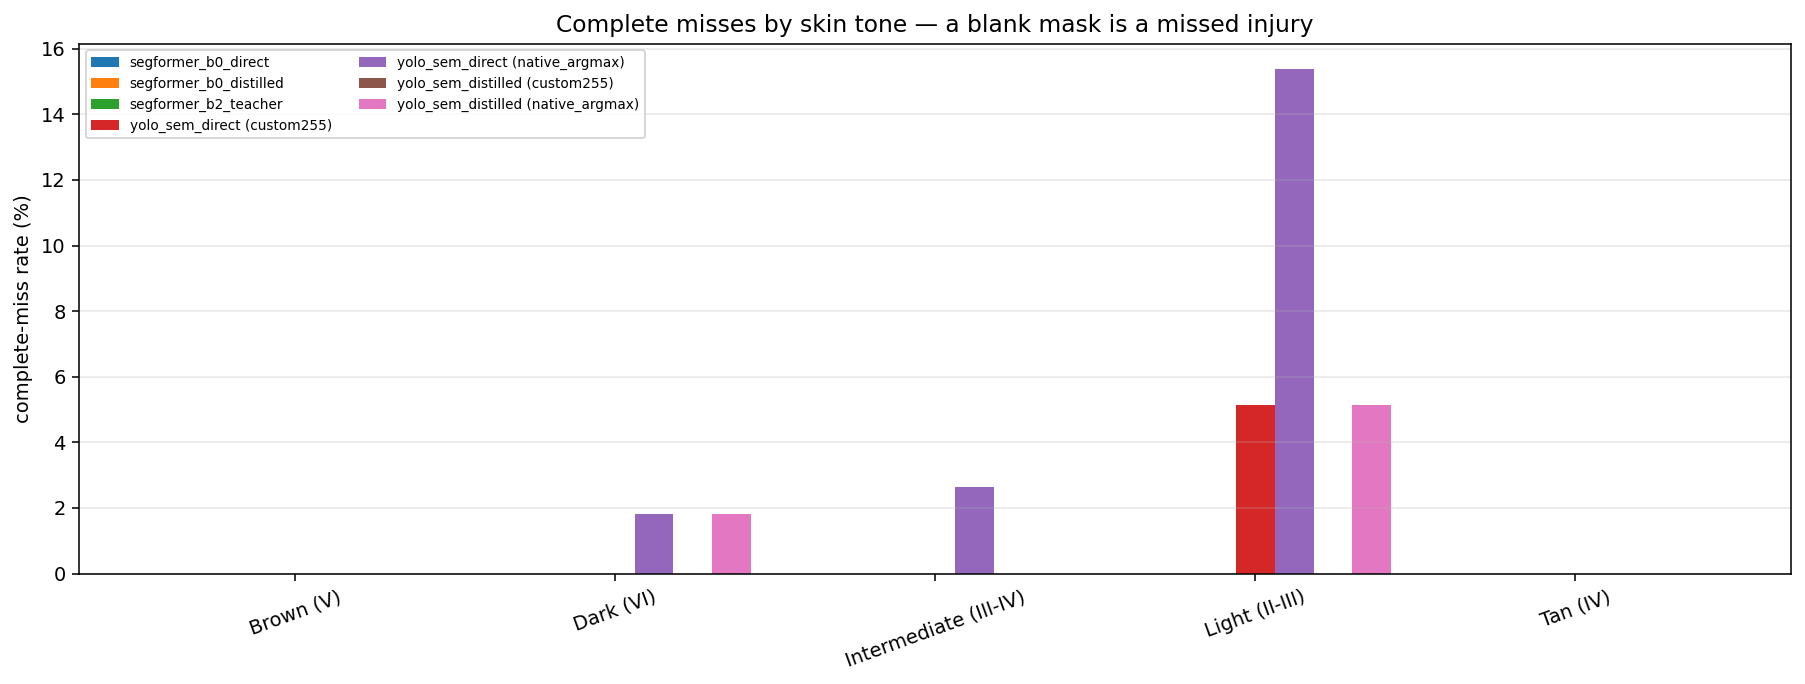
\includegraphics[width=0.92\linewidth]{figures/final_fairness_miss.png}
\caption{Complete-miss rate by ITA skin-tone group (three-seed). SegFormer
variants sit at zero across groups; the YOLO variants concentrate their misses on
the lightest-skin group.}
\label{fig:miss}
\end{figure}

% ======================================================================
\section{Results: Bruise Size, and the Size--Fairness Confound}
% ======================================================================
Small bruises are intrinsically harder---a few pixels of boundary error cost
proportionally more Dice on a small target, and misses concentrate on the
smallest lesions. This matters for Section~\ref{sec:fairness} because
\textbf{lesion size is confounded with skin tone in this cohort}. Median bruise
size by ITA group: Light (II--III) \textbf{8{,}085}\,px, Brown 10{,}961, Intermediate
12{,}118, Tan 13{,}550, Dark 13{,}751. Light-skin bruises are $\approx$33\% smaller
than the median of the rest (Kruskal--Wallis $H=21.1$, $p=0.0003$).

\subsection{Does the skin-tone signal survive size?}
We test this directly, with \textbf{standard errors clustered by subject}
(treating 185 images as independent would badly overstate significance for a
9-subject group). Two findings:

\begin{itemize}[leftmargin=1.4em]
\item \textbf{Stratified.} Within the smallest size tercile of YOLO-direct
      (where size is roughly held fixed), the light-skin group still fares worse:
      complete-miss \textbf{30\%} vs.\ \textbf{9.5\%}, mean recall \textbf{0.41}
      vs.\ \textbf{0.69}. The gap does not vanish under size control.
\item \textbf{Regression.} In $\texttt{recall} \sim \log_{10}(\text{size}) +
      \text{light}$ with subject-clustered SEs, the light coefficient is
      $-0.176$ ($p=0.047$) for YOLO-direct and $-0.164$ ($p=0.045$) for
      YOLO-distilled, while $\log(\text{size})$ is itself non-significant---so the
      light-skin recall deficit is \emph{not only} size. For the binary
      complete-miss outcome the light term is non-significant once size is in
      ($p=0.62$); it is the graded recall, not the blank-mask event, that carries
      the residual signal. The SegFormer models show no light-skin effect
      ($p>0.39$).
\end{itemize}

Clustering is decisive here: the naive, image-independent version of the same
recall regression gives $p=0.0016$, an order of magnitude smaller than the honest
$p=0.047$. The contrast is itself a clean illustration of benchmark fragility.
\textbf{Net reading:} the apparent skin-tone gap is partly a size artefact, but a
residual light-skin recall deficit for YOLO survives size and clustering at the
boundary of significance. At 9 light-skin subjects this is a hypothesis to test on
more data, not a proven disparity.

% ======================================================================
\section{Discussion}
% ======================================================================
Three themes recur. \textbf{(1) Label-limited, not capacity-limited.} All
transformer variants---\emph{and} the U-Net / DeepLabV3+ CNN baselines
(Section~\ref{sec:baselines})---sit within a Dice band (0.745--0.765) narrower than
human--human disagreement; seven architectures cluster there, and the binding constraint is
annotation noise (Section~\ref{sec:ceiling}), not model capacity. \textbf{(2) Miss rate is the honest axis.} It is the
one quantity that separates architectures by more than label noise and the one
that matters clinically; SegFormer is essentially miss-free while YOLO is not.
\textbf{(3) Benchmark fragility.} The headline numbers move more with
harness choices---subject vs.\ image resampling, evaluation path (YOLO native vs.\
custom), preprocessing, batch/step budget---than with architecture. A study that
reports a single accuracy number, treats images as independent, or fixes a
threshold at 0.5 would draw materially different (and less defensible)
conclusions.

\paragraph{Deployment and licensing.} For a non-commercial forensic tool both
model families are usable, but the licenses differ: the SegFormer pretrained
weights carry an NVIDIA non-commercial license, and Ultralytics/YOLO is AGPL-3.0
(network copyleft; reimplementing the code does not free the weights). On both
accuracy-safety (misses) and license risk, SegFormer is the preferable deployment
target, with YOLO retained as a fast baseline.

% ======================================================================
\section{Limitations}
% ======================================================================
\label{sec:limits}
\begin{itemize}[leftmargin=1.4em]
\item \textbf{Sample size is a hard ceiling.} $n=28$ subjects is the maximum for
      which three-annotator consensus labels exist; the minimum resolvable mean-Dice
      effect is $\approx$0.04.
\item \textbf{Unequalised training budget.} With per-model batch, the B2 teacher
      trains $\approx$2100 steps vs.\ $\approx$1000 for each B0 student
      (Table~\ref{tab:batch})---a confound in the teacher--student comparison.
      A batch-matched run (effective batch 8 for all) exists separately and could
      be used to isolate architecture from budget.
\item \textbf{Single site, single modality} (white light), single annotator for
      training (Paul).
\item \textbf{Fairness is exploratory} ($\approx$9--17 subjects/group); the
      size--skin-tone confound is real and only partially resolved.
\item \textbf{Single-seed inference} for the analysis figures (the best
      validation seed); three-seed aggregates are reported for the headline tables.
\end{itemize}

% ======================================================================
\section{External Baselines: U-Net and DeepLabV3+}
% ======================================================================
\label{sec:baselines}
Two external baselines were trained in \texttt{bruise\_colab\_baselines.ipynb} through the
\emph{identical} SegFormer shared recipe (they are plain \texttt{nn.Module}s: an
ImageNet-pretrained ResNet50 encoder + a randomly-initialised decoder, so the shared recipe
is fair), on the same 697/134 split, \textbf{seeds 0/1/2}, scored against the same 2-of-3
majority target at 640 with complete-miss rate reported. Results are the three-seed
mean$\pm$std in Table~\ref{tab:baselines}. \emph{(nnU-Net v2, the native self-configuring
``each-at-its-strongest'' datapoint, has not been run yet; it will be added later.)}

\begin{table}[h]
\centering
\caption{External baseline results (3 seeds, 185 test images), next to the core SegFormer
models for context. All trained with the shared recipe; scored vs the 2-of-3 majority @640.}
\label{tab:baselines}
\begin{tabular}{lcccc}
\toprule
Model & Params (M) & Mean Dice & Median Dice & Miss \% \\
\midrule
SegFormer-B2 teacher \emph{(core)}    & 27.35 & 0.765 $\pm$ 0.004 & 0.811 & 0.00 \\
SegFormer-B0 direct \emph{(core)}     & 3.71  & 0.760 $\pm$ 0.006 & 0.811 & 0.54 \\
\midrule
\textbf{U-Net (ResNet50)}      & 32.52 & \best{0.753 $\pm$ 0.015} & 0.826 & 3.24 $\pm$ 0.54 \\
\textbf{DeepLabV3+ (ResNet50)} & 26.68 & \best{0.745 $\pm$ 0.018} & 0.814 & 1.80 $\pm$ 0.62 \\
nnU-Net v2 (2d)                & --- & \emph{pending} & \emph{pending} & \emph{pending} \\
\bottomrule
\end{tabular}
\end{table}

\paragraph{The baselines reinforce the annotation-ceiling thesis.} With U-Net and
DeepLabV3+ added, \textbf{seven architectures now span roughly 0.745--0.765 mean Dice}
(SegFormer 0.760--0.765, U-Net 0.753, DeepLabV3+ 0.745; the YOLO family lower at
0.69--0.73). U-Net in particular is statistically indistinguishable from the SegFormer-B0
students: the point gap SegFormer-B0-direct $-$ U-Net is only $\approx$0.007, and even
SegFormer-B2 $-$ DeepLabV3+ is $\approx$0.020---both at or below the $\approx$0.04 minimum
detectable effect at $n=28$. This is exactly the pattern the label-limited hypothesis
predicts: swapping a transformer for a CNN, or U-Net for DeepLabV3+, moves Dice less than
the annotation noise. \textbf{We therefore do not claim ``SegFormer beats U-Net/DeepLabV3+''}
on Dice.

\paragraph{Miss rate still orders the architectures the same way.} The safety axis is again
more informative than Dice: SegFormer ($0$--$0.5\%$) $<$ DeepLabV3+ ($1.80\%$) $<$ U-Net
($3.24\%$) $<$ YOLO ($2$--$8\%$). The transformer remains the safest; among the CNN
baselines, DeepLabV3+'s ASPP context gives it a lower blank-mask rate than U-Net.

\paragraph{Fairness (baselines).} Neither baseline shows a significant ITA effect
(Kruskal--Wallis $p=0.22$ U-Net, $p=0.11$ DeepLabV3+; best$-$worst-group median-Dice gap
$0.096$ and $0.079$), consistent with the exploratory-at-$n{=}28$ reading of
Section~\ref{sec:fairness}. Per-group medians are in Figure~\ref{fig:base_fair}.

\begin{figure}[h]
\centering
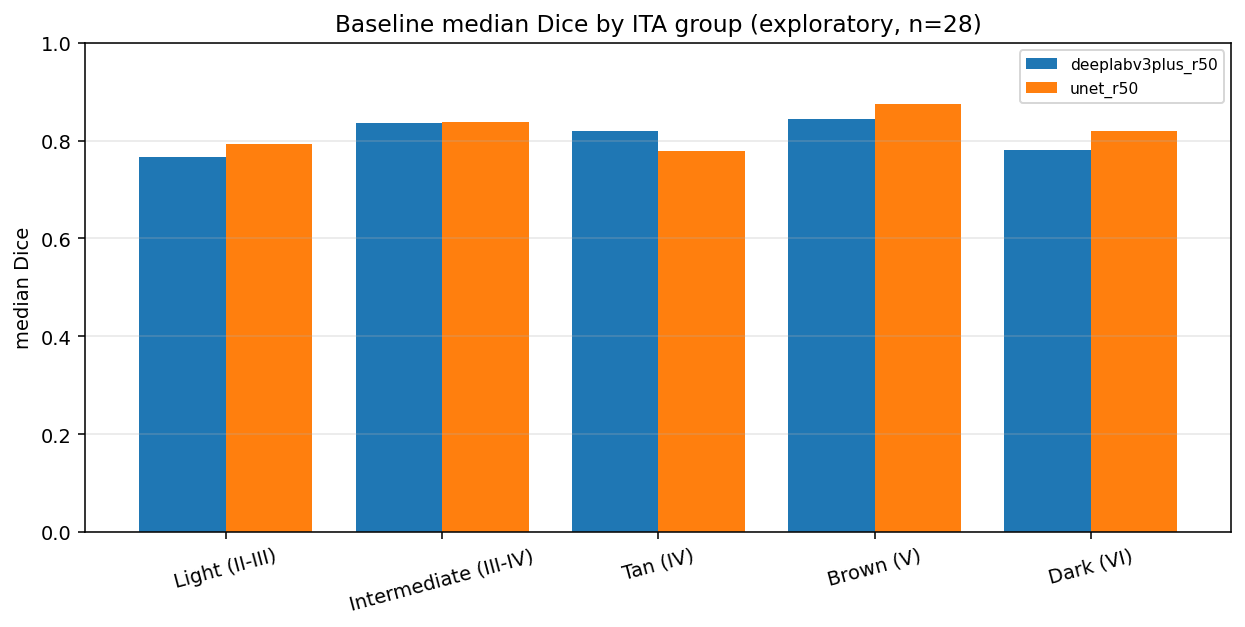
\includegraphics[width=0.78\linewidth]{figures/baselines_fairness_by_group.png}
\caption{Baseline median Dice by ITA skin-tone group (three-seed; exploratory at $n=28$).}
\label{fig:base_fair}
\end{figure}

\paragraph{Best-seed selection (parity with the core best-seed table).} To compare the
baselines on the \emph{same} policy as Table~\ref{tab:best}---best seed chosen on
\emph{validation} Dice, then scored on test---each baseline's best of three seeds was
selected from its saved validation operating point (\texttt{operating\_point.json}); results
in Table~\ref{tab:baselines_best}. The val-selected baselines rise slightly (best-of-3 vs.\
mean-of-3) but the ordering is unchanged: both sit below the three SegFormer models on mean
Dice and blank more often. Notably U-Net posts the \emph{highest median Dice of any model}
(0.833), yet its larger mean--median gap and 3.78\% miss rate reflect more complete
failures---the same median-is-not-safety lesson as YOLO.

\begin{table}[h]
\centering
\caption{Baselines, best seed selected on validation Dice (same policy as
Table~\ref{tab:best}); that seed's test result reported.}
\label{tab:baselines_best}
\begin{tabular}{lcccc}
\toprule
Model & Params (M) & Test mean Dice & Test median Dice & Miss \% \\
\midrule
DeepLabV3+ (ResNet50) & 26.68 & 0.758 & 0.818 & 2.16 \\
U-Net (ResNet50)      & 32.52 & 0.757 & 0.833 & 3.78 \\
\bottomrule
\end{tabular}
\end{table}

\paragraph{The paired bootstrap is now unblocked.} The per-image test scores needed for a
paired subject-level cluster-bootstrap of each baseline against the core models
(as in Table~\ref{tab:paired}) are available in
\texttt{runs\_baselines/*/test\_per\_image.csv}; each baseline-vs-core comparison should be
reported as $\Delta$ mean/median Dice + 95\% CI + $P(\Delta{>}0)$. Given the point gaps
($\approx$0.007--0.020, all at or below the $\approx$0.04 minimum detectable effect at
$n=28$), most are expected to be n.s.

% ======================================================================
\section{Reproducibility and Artifacts}
% ======================================================================
\begin{itemize}[leftmargin=1.4em]
\item \textbf{Training/eval:} \texttt{bruise\_colab\_final.ipynb}
      (generator \texttt{scripts/43\_generate\_final\_notebook.py}); five models,
      three seeds, native YOLO, two YOLO eval paths, ITA fairness. Outputs in
      \texttt{results\_final/} and checkpoints in \texttt{runs\_final/}.
\item \textbf{Analysis:} \texttt{bruise\_colab\_final\_analysis.ipynb}
      (generator \texttt{scripts/44\_generate\_final\_analysis\_notebook.py});
      best-seed re-inference, $\approx$25 figures, annotation ceiling,
      model-vs-Paul, paired contrasts with $P(\Delta{>}0)$, ITA fairness, bruise
      size, and the size-conditioned regression of
      Section~\ref{sec:baselines}--10.
\item \textbf{Baselines:} \texttt{bruise\_colab\_baselines.ipynb}
      (generator \texttt{scripts/45\_generate\_baselines\_notebook.py}).
\item All numeric results in this report are read directly from the run CSVs
      (\texttt{FINAL\_RESULTS.csv}, \texttt{*\_test\_per\_seed.csv},
      \texttt{benchmark\_640.csv}, \texttt{fairness\_*.csv}) and the analysis
      outputs (\texttt{final\_analysis\_*/}); none are transcribed by hand.
\end{itemize}

% ======================================================================
\section*{Key references}
% ======================================================================
\small
\sloppy
\begin{itemize}[leftmargin=1.4em, itemsep=1pt]
\item Xie et al., \emph{SegFormer: Simple and Efficient Design for Semantic
      Segmentation with Transformers}, NeurIPS 2021.
\item Jocher et al., \emph{YOLO26}, arXiv:2606.03748, 2026.
\item Guo et al., \emph{On Calibration of Modern Neural Networks}, ICML 2017
      (temperature scaling).
\item Menon et al., \emph{A Statistical Perspective on Distillation}, ICML 2021
      (calibrated soft-target distillation; the formula used here).
\item Milletari et al., \emph{V-Net} (Dice loss), 3DV 2016; Drozdzal et al.\ 2016
      (Dice$+$BCE).
\item Chardon et al., \emph{Individual Typology Angle}, 1991 (objective skin tone).
\item Efron \& Tibshirani, \emph{An Introduction to the Bootstrap}, 1993
      (cluster/percentile bootstrap).
\end{itemize}

\end{document}
